\section{Příklad 1}
% Jako parametr zadejte skupinu (A-H)
\prvniZadani{H}
\subsection{Zjednodusovanie}
$R_3$ a $R_4$ su zapojene paralelne - mozeme ich nahradit za $R_{34} = \frac{R_3 \cdot R_4}{R_3 + R_4} = \SI{141.4035088}{\ohm}$
\begin{figure}[!h]
    \centering
    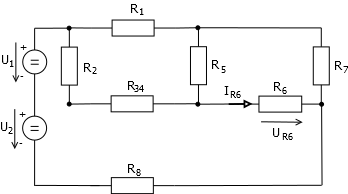
\includegraphics[width=0.5\linewidth]{pr1/2.png}
 \end{figure}
 
$R_2$ a $R_{34}$ su zapojene seriovo - mozeme ich nahradit za $R_{234} = R_2 + R_{34} = \SI{741.4035088}{\ohm}$
\begin{figure}[!h]
    \centering
    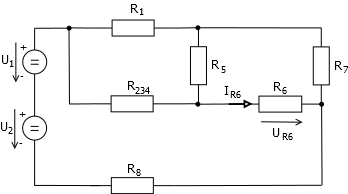
\includegraphics[width=0.5\linewidth]{pr1/3.png}
\end{figure}
\newpage

Z $R_{1}$, $R_{234}$, $R_{5}$ nam vznikol trojuholnik - pouzijeme transfiguraciu trojuholnik -> hviezda
\begin{align*}
    R_A = \frac{R_1 \cdot R_{234}}{R_1 + R_5 + R_234} &= 252.5315063\\
    R_B = \frac{R_1 \cdot R_{5}}{R_1 + R_5 + R_234} &= 195.8521903\\
    R_C = \frac{R_5 \cdot R_{234}}{R_1 + R_5 + R_234} &= 213.5375017\\
\end{align*}
\begin{figure}[!h]
    \centering
    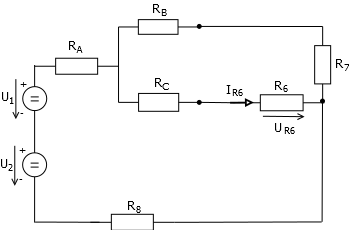
\includegraphics[width=0.5\linewidth]{pr1/4.png}
\end{figure}

$R_C$ a $R_{6}$ su zapojene seriovo - mozeme ich nahradit za $R_{C6} = R_C + R_{6} = \SI{1083.5375017}{\ohm}$\\
$R_B$ a $R_{7}$ su zapojene seriovo - mozeme ich nahradit za $R_{C6} = R_B + R_{7} = \SI{550.8521903}{\ohm}$
\begin{figure}[!h]
    \centering
    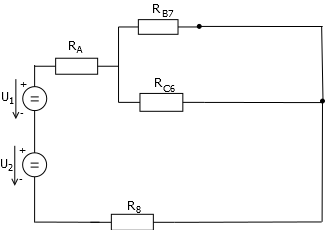
\includegraphics[width=0.5\linewidth]{pr1/5.png}
\end{figure}

$R_B7$ a $R_C6$ su zapojene paralelne - mozeme ich nahradit za $R_{B7C6} = \frac{R_{B7} \cdot R_{C6}}{R_{B7} + R_{C6}} = \SI{365.1938145}{\ohm}$
\begin{figure}[!h]
    \centering
    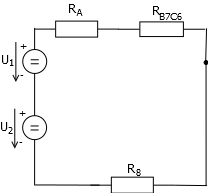
\includegraphics[width=0.2\linewidth]{pr1/6.png}
\end{figure}
\newpage

$R_A$, $R_{B7C7}$ a $R_{8}$ su zapojene seriovo - mozeme ich nahradit za \\
$R_{ekv} = R_A + R_{B7C7} + R_{8} = \SI{882.7253208}{\ohm}$\\
Zdroje $U_1$ a $U_2$ su tiez zapojene seriovo - nahradime ich za $U_{12} = U_1 + U_2 = \SI{215}{\volt}$
\begin{figure}[!h]
    \centering
    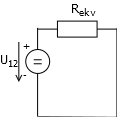
\includegraphics[width=0.2\linewidth]{pr1/7.png}
\end{figure}

\subsection{Spatny vypocet}
Teraz uz lahko vypocitame celkovy prud pretekajuci obvodom. Tiez sa vieme spatne prepocitat az k hladanemu $U_{R6}$ a $I_{R6}$.

\begin{align*}
    I_{ekv} = \frac{U_{12}}{R_{ekv}} &= \frac{\SI{215}{\volt}}{\SI{882.7253208}{\ohm}} = \SI{0.243563875}{\ampere}\\
    U_{B7C6} = I_{ekv} \cdot R_{B7C6} &= \SI{0.243563875}{\ampere} \cdot \SI{365.1938145}{\ohm} = \SI{88.94802058}{\volt}\\
    U_{C6} = U_{B7} &= U_{B7C6} = \SI{88.94802058}{\volt}\\
    I_{C6} = \frac{U_{C6}}{R_{C6}} &= \frac{\SI{88.94802058}{\volt}}{\SI{1083.5375017}{\ohm}} = \SI{0.082090394}{\ampere}\\
    I_6 = I_{C6} &= \SI{0.082090394}{\ampere}\\
    U_{6} = I_{6} \cdot R_{6} &= \SI{0.082090394}{\ampere} \cdot \SI{870}{\ohm} = \SI{71.41864290}{\volt}\\
\end{align*}